\documentclass[]{book}

%These tell TeX which packages to use.
\usepackage{array,epsfig}
\usepackage{amsmath}
\usepackage{amsfonts}
\usepackage{amssymb}
\usepackage{amsxtra}
\usepackage{amsthm}
\usepackage{mathrsfs}
\usepackage{color}

%Here I define some theorem styles and shortcut commands for symbols I use often
\theoremstyle{definition}
\newtheorem{defn}{Definition}
\newtheorem{thm}{Theorem}
\newtheorem{cor}{Corollary}
\newtheorem*{rmk}{Remark}
\newtheorem{lem}{Lemma}
\newtheorem*{joke}{Joke}
\newtheorem{ex}{Example}
\newtheorem*{soln}{Solution}
\newtheorem{prop}{Proposition}

\newcommand{\lra}{\longrightarrow}
\newcommand{\ra}{\rightarrow}
\newcommand{\surj}{\twoheadrightarrow}
\newcommand{\graph}{\mathrm{graph}}
\newcommand{\bb}[1]{\mathbb{#1}}
\newcommand{\Z}{\bb{Z}}
\newcommand{\Q}{\bb{Q}}
\newcommand{\R}{\bb{R}}
\newcommand{\C}{\bb{C}}
\newcommand{\N}{\bb{N}}
\newcommand{\M}{\mathbf{M}}
\newcommand{\m}{\mathbf{m}}
\newcommand{\MM}{\mathscr{M}}
\newcommand{\HH}{\mathscr{H}}
\newcommand{\Om}{\Omega}
\newcommand{\Ho}{\in\HH(\Om)}
\newcommand{\bd}{\partial}
\newcommand{\del}{\partial}
\newcommand{\bardel}{\overline\partial}
\newcommand{\textdf}[1]{\textbf{\textsf{#1}}\index{#1}}
\newcommand{\img}{\mathrm{img}}
\newcommand{\ip}[2]{\left\langle{#1},{#2}\right\rangle}
\newcommand{\inter}[1]{\mathrm{int}{#1}}
\newcommand{\exter}[1]{\mathrm{ext}{#1}}
\newcommand{\cl}[1]{\mathrm{cl}{#1}}
\newcommand{\ds}{\displaystyle}
\newcommand{\vol}{\mathrm{vol}}
\newcommand{\cnt}{\mathrm{ct}}
\newcommand{\osc}{\mathrm{osc}}
\newcommand{\LL}{\mathbf{L}}
\newcommand{\UU}{\mathbf{U}}
\newcommand{\support}{\mathrm{support}}
\newcommand{\AND}{\;\wedge\;}
\newcommand{\OR}{\;\vee\;}
\newcommand{\Oset}{\varnothing}
\newcommand{\st}{\ni}
\newcommand{\wh}{\widehat}

%Pagination stuff.
\setlength{\topmargin}{-.3 in}
\setlength{\oddsidemargin}{0in}
\setlength{\evensidemargin}{0in}
\setlength{\textheight}{9.in}
\setlength{\textwidth}{6.5in}
\pagestyle{empty}



\begin{document}


\begin{center}
{\textbf{Magma viscosity and density}}\\
Paul A. Jarvis\\ %You should put your name here
\end{center}

\vspace{0.2 cm}


\begin{enumerate}
  %Question 1%%%%%%%%%%%%%%%%%%%%%%%%%%%
\item Table~\ref{tab:comp} lists bulk rock compositions as measured for erupted lavas from various volcanoes. 

  \begin{table}
    \centering
    \caption{Dry, bulk rock compositions for various volcanoes (wt\%). Two different lavas were erupted at Unzen in the 1991-1995 eruption. \label{tab:comp}}
    \begin{tabular}{|c|c|c c c c c c c c c c c|}
      \hline
      Volcano & Eruption & SiO$_{2}$ & Al$_{2}$O$_{3}$ & TiO$_{2}$ & FeO & Fe$_{2}$O$_{3}$ & MnO & MgO & CaO & K$_{2}$O & Na$_{2}$O & P$_{2}$O$_{5}$ \\
      \hline
      Unzen$^{1}$ & 1991-1995 & 64.27 & 16.13 & 0.71 & 0.00 & 5.10 & 0.10 & 2.47 & 4.69 & 2.54 & 3.81 & 0.17 \\
      Unzen$^{2}$ & 1991-1995 & 51.84 & 18.19 & 1.28 & 0.00 & 10.27 & 0.18 & 4.62 & 9.43 & 1.22 & 2.79 & 0.17 \\
      Kilauea & 1992 & 49.78 & 12.79 & 2.37 & 0.00 & 12.40 & 0.17 & 8.75 & 10.59 & 0.41 & 2.14 & 0.22 \\
      MORB & N/A & 50.47 & 14.70 & 1.68 & 10.43 & 0.00 & 0.18 & 7.58 & 11.39 & 0.16 & 2.79 & 0.18 \\
      Novarupta & 1912 & 77.19 & 12.28 & 0.18 & 1.3 & 0.0 & 0.05 & 0.19 & 0.87 & 3.17 & 4.32 & 0.05 \\
      \hline
    \end{tabular}
  \end{table}

  \begin{enumerate}
  \item Use Figure~\ref{fig:TAS} to classify the composition of the rocks in Table~\ref{tab:comp}. 
  \item Create a new table listing the compositions shown in Table~\ref{tab:comp}, but presenting the data in mol\%
  \end{enumerate}

  \begin{figure}
    $$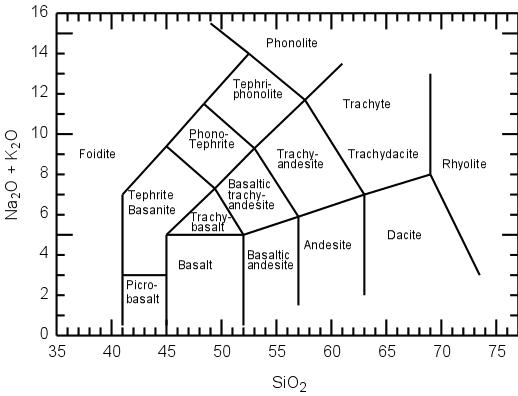
\includegraphics[width=\textwidth]{TAS.JPG}$$
    \caption{Total Alkali-Silica (TAS) diagram for characterisation of volcanic rocks. \label{fig:TAS}}
  \end{figure}

  Table~\ref{tab:liq} shows the liquidus temperatures of the magmas in Table~\ref{tab:comp} for both dry composition and 4 wt\% water at 200 MPa.

  \begin{enumerate}\setcounter{enumii}{2}
  \item For the Novarupta volcano, determine the wet melt composition at the wet liquidus temperature at 200 MPa. 
\end{enumerate}

  Furthermore, the volume $V_{\text{m}}$ of 1 mol of melt of composition $\mathbf{X}$ as a function of pressure $P$ and temperature $T$ is given by

  \begin{align}
    \label{equ:mol_vol}
    V_{m}(T, P, \mathbf{X}) = \sum_{i} X_{i} \Bigg[ \textcolor{red}{\bar{V_{i}}(T = T_{\text{R}}, P = P_{\text{R}})} & + \left. \textcolor{blue}{\left. \frac{\partial \bar{V_{i}}(T, P = P_{\text{R}})}{\partial T}\right|_{T = T_{\text{R}}}} (T - T_{\text{R}}) \right. \nonumber \\
      & + \left. \textcolor{green}{\left.\frac{\partial \bar{V_{i}}(T = T_{\text{R}}, P)}{\partial P}\right|_{P = P_{R}}} (P - P_{\text{R}})\right], 
  \end{align}

  where $T_{\text{R}} = 1673$ K and $P_{\text{R}} = 10^{-4}$ GPa. Values for the red, blue and green quantities can be found in Table~\ref{tab:mol_vol}.
  
  \begin{table}
    \centering
    \caption{Liquidus tempertaures for rocks show in Table~\ref{tab:comp} at 200 MPa for dry and wet (4 wt\% water) compositions. \label{tab:liq}}
    \begin{tabular}{|c|c|c|c|}
      \hline
      Volcano & Eruption & Dry Liquidus $T$ /$^{\circ}$C & Wet Liquidus $T$ /$^{\circ}$C  \\
      \hline
      Unzen$^{1}$ & 1991-1995 & 1148 & 1043 \\
      Unzen$^{2}$ & 1991-1995 & 1226 & 1079 \\
      Kilauea & 1992 & 1237 & 1172 \\
      MORB & N/A & 1215 & 1145 \\
      Novarupta & 1912 & 1123 & 826.56 \\
      \hline
    \end{tabular}
  \end{table}

  \begin{table}
    \centering
    \caption{Partial molar volume, thermal expansions and compressibilities of oxide components \label{tab:mol_vol}}
    \begin{tabular}{|c|c|c|c|}
      \hline
      & $\textcolor{red}{\bar{V_{i}}(T = T_{\text{R}}, P = P_{\text{R}})}$ & $\textcolor{blue}{\left.\frac{\partial \bar{V_{i}}(T, P = P_{\text{R}})}{\partial T}\right|_{T = T_{\text{R}}}}$ & $\textcolor{green}{\left.\frac{\partial \bar{V_{i}}(T = T_{\text{R}}, P)}{\partial P}\right|_{P = P_{R}}}$ \\
      & /10$^{-6}$ m$^{3}$ mol$^{-1}$ & /10$^{-9}$ m$^{3}$ mol$^{-1}$ K & /10$^{-6}$ m$^{3}$ mol$^{-1}$ GPa \\
      \hline
      SiO$_{2}$ & 26.86 & 0.0 & -1.89 \\
      TiO$_{2}$ & 23.16 & 7.24 & -2.31 \\
      Al$_{2}$O$_{3}$ & 37.42 & 0.0 & -2.31 \\
      Fe$_{2}$O$_{3}$ & 42.13 & 9.09 & -2.53 \\
      FeO & 13.65 & 2.92 & -0.45 \\
      MgO & 11.69 & 3.27 & 0.27 \\
      CaO & 16.53 & 3.74 & 0.34 \\
      Na$_{2}$O & 28.88 & 7.68 & -2.40 \\
      K$_{2}$O & 45.07 & 12.08 & -6.75 \\
      Li$_{2}$O & 16.85 & 5.25 & -1.02 \\
      H$_{2}$O & 26.27 & 9.46 & -3.15 \\
      CO$_{2}$ & 33.0 & 0.0 & 0.0 \\
      \hline  
    \end{tabular}
  \end{table}

  \begin{enumerate}\setcounter{enumii}{3}
  \item For the Novarupta volcano, determine the density of the \textbf{dry} melt composition at the \textbf{dry} liquidus temperature, at 200 MPa. Take care with units and show your method clearly (it may be helpful to draw a table). 
  \item For the same volcano, determine the density of the \textbf{wet} melt composition at the \textbf{dry} liquidus temperature, at 200 MPa.
  \item Again for Novarupta, determine the density of the \textbf{wet} melt composition at the \textbf{wet} liquidus temperature, at 200 MPa.
  \item Describe the effect of both temperature and water content on the density of the magmatic melt at Novarupta. Be as quantitative as you can.
  \end{enumerate}

  %Question 2%%%%%%%%%%%%%%%%%%%%%%%%%%%

\item At a temperature of 767 $^{\circ}$C and pressure of 200 MPa, the equilibrium crystal assemblage of the wet Novarupta magma is feldspar ($\phi_{\text{fld}} = 0.5, \rho_{\text{fld}} = 2.5$ g cm$^{-3}$), quartz ($\phi_{\text{qz}} = 0.3, \rho_{\text{qz}} = 2.5$ g cm$^{-3}$), spinel ($\phi_{\text{sp}} = 0.007, \rho_{\text{sp}} = 4.9$ g cm$^{-3}$) and biotite ($\phi_{\text{bio}} = 0.5, \rho_{\text{bio}} = 2.75$ g cm$^{-3}$) whilst the melt density is 2.21 g cm$^{-3}$ and the melt viscosity is 147910.8 Pa s. Additionally, the gravitational settling velocity of a crystal of size $d$ and density $\rho_{\text{c}}$ in melt of density $\rho_{\text{m}}$ and viscosity $\eta_{\text{m}}$ is given by

  \begin{equation}
    \label{equ:Stokes}
    v_{\text{s}} = \frac{(\rho_{\text{c}} - \rho_{\text{m}}) g d^{2}}{18 \eta_{\text{m}}},
  \end{equation}

  where $g = 9.81$ m s$^{-1}$ is the gravitational acceleration. 

  \begin{enumerate}
    \setcounter{enumi}{1}
  \item Calculate the settling velocities of each crystal phase in the Novarupta magma.
  \end{enumerate}

  For the wet Kilauea composition, the equilibrium assemblage at the same pressure is olivine ($\phi_{\text{ol}} = 0.03, \rho_{\text{ol}} = 3.37$ g cm$^{-3}$), orthopyroxene ($\phi_{\text{opx}} = 0.006, \rho_{\text{fld}} = 3.28$ g cm$^{-3}$), clinopyroxene ($\phi_{\text{cpx}} = 8.21, \rho_{\text{cpx}} = 3.29$ g cm$^{-3}$) and spinel ($\phi_{\text{sp}} = 0.02, \rho_{\text{sp}} = 4.9$ g cm$^{-3}$), with a melt density of 2.31 g cm$^{-3}$ and a melt viscosity of 28.1 Pa s. 

  \begin{enumerate}
    \setcounter{enumi}{2}
  \item Calculate the settling velocities of each crystal phase in the Kilauea magma.
  \item It has been suggested that crystal cumulates can form at the base of magma chambers of sills by gravitational settling of crystals. Consider 10 m thick sills of both the Novarupta and Kilauea compositions. If the sills were maintained at constant temperatures, how long would it take for such a cumulate to form in each case?
  \item What are the most important parameters in determining whether such cumulates can form? Also consider processes which have been neglected here.
  \end{enumerate}
  
\end{enumerate}
\end{document}
